% Thesis template by Aleksander M. Stensby
% aleksander.stensby@gmail.com

\documentclass[12pt,letterpaper,final]{report}
%\documentclass[12pt,a4paper,final]{report}
\usepackage{makeidx}
\usepackage{varioref}
\usepackage{setspace}
\usepackage{times} % Use this package for times-font. %%not found
\usepackage{fancyvrb}
\usepackage{moreverb}
\usepackage{fancyhdr}
\usepackage{epsfig}
\usepackage{eucal}
\usepackage{amsmath}
\usepackage{amsfonts}
\usepackage{floatflt}
\usepackage{tocbibind}
\usepackage{wrapfig}
\usepackage{listings}
\usepackage{color}
\usepackage{amsthm}
\usepackage{subfigure}
\usepackage{longtable}
\usepackage{url}
\usepackage{multicol}
\usepackage{array}
\usepackage[style=list,toc=true]{glossaries}
\usepackage{graphicx} %For � kunne inkludere grafikk
\usepackage{hiafrontpage} % For UoA Style frontpage.
\usepackage{rotating}

\definecolor{Brown}{cmyk}{0,0.81,1,0.60}
\definecolor{OliveGreen}{cmyk}{0.64,0,0.95,0.40}
\definecolor{Keyword}{cmyk}{0.66,0.90,0.33,0.20}
\definecolor{Comment}{cmyk}{0.88,0.35,1.00,0.30}
\definecolor{Identifier}{cmyk}{1,1,1,1}
\definecolor{XmlKeyword}{cmyk}{0.66,0.90,0.33,0.20}
\definecolor{FrameColor}{cmyk}{0.66,0.90,0.33,0.20}
\definecolor{XmlIdentifier}{cmyk}{0,0.81,1,0.60}
\definecolor{XmlString}{cmyk}{1,1,1,1}


%%%% Fancy
% 11pt font
%\headheight=13.6 pt

% 12pt font
\headheight=14.5 pt

\pagestyle{fancy} 
\fancyhead[L]{\leftmark}
\fancyhead[R]{}
%lowercase
%\renewcommand{\chaptermark}[1]{\markboth{#1}{}}

%Fit more figures on a page
\renewcommand{\topfraction}{.99}
\renewcommand{\bottomfraction}{.99}
\renewcommand{\textfraction}{.01}
\renewcommand{\floatpagefraction}{.99}

% spacing:
%\singlespacing
\onehalfspacing
%\doublespacing

\theoremstyle{definition}
\newtheorem{theorem}{Theorem}
\hyphenation{theorem}
\newtheorem{definition}{Definition}
\newtheorem{remark}{Remark}

\oddsidemargin=0.5in \evensidemargin=0.3in
\parskip=0.0 true in

\author{Haakon Bakkevig Steinsholt and Daniel Aasen}
\supervisor{Morten Goodwin and Ole-Christoffer Granmo}
\titlelogo{images/uia_logo_large} %Path to UoA logo.
\title{Examining Ant Colony Optimization Performance for Ship Evacuation}

\draftversion{3.6}
%\date{January 9, 2007} %specify own date

\makeglossary

%for draft work, select the chapters to include in the pdf but still keep all cross-references intact.
%\includeonly{introduction}

\begin{document}

    \maketitle

    \newpage    
    \begin{abstract}

Evacuating passengers during a fire on board a ship is a difficult task and any improvements on current procedures can help save lives. This report describes how an Ant Colony Optimization (ACO) pathfinding algorithm could possibly be used to lead passengers out of this dangerous situation. The ships were modeled as graphs with nodes and vertices. In the simulation passengers were equipped with a smart phone running an application which showed them the way out. The passengers could end up panicking given close proximity to fire or other stressing factors, in which case they would stop following directions. Additionally, high density of passengers in rooms and corridors slowed down the speed of evacuation.  The results produced by ACO were compared to Dijkstra's pathfinding algorithm and were promising. They showed that ACO performed well in dynamic environments and could be used in a crisis situation to guide people out of danger.

\end{abstract}

    % \chapter*{Preface}

Your preface goes here.

    \tableofcontents
    \listoffigures
    \listoftables

    \parskip=0.1 true in

    \newpage

		% General structure, normally (background, and solution chapter may be split into several different chapters!
    \chapter{Introduction}
\label{ch:introduction}

\section{Introduction}

A fire on board a ship can have disastrous consequences, and as good as the evacuation plans may be now,                           
they will need improvement to ensure that as many passengers as possible survives. This project will work                           
 on modifying existing algorithms that will attempt to find the optimal path of evacuation during a simulated crisis, and which could         
 one day be used to help save lives during a crisis that otherwise may have been lost. 

Our main focus is the Ant Colony Optimization, a pathfinding algorithm which finds a path through
 the environment to the desired destination by mimicking the behavior of an ant colony. The algorithm sends    
out virtual ants that search for a valid path then report back the path they took.            
These paths are marked with pheromones and any consecutive ants are more likely to walk on the previously successful paths.

In this thesis we will compare Dijkstra's pathfinding algorithm to ACO, as Dijkstra's is one of the most commonly
 used pathfinding algorithms today. We will model the ship as a dynamic graph with nodes and edges where
 the nodes can be rooms, hallways or other sections of the ships and the edges indicate that it is possible to
 transition from one node to another. The simulated passengers will receive directions on their smart phones.

Additionally, we will simulate human behavior during a crisis and observe
 how this affects the algorithms. Finally we will look into how high occupant density around exits slow down the 
evacuation process and explore how to redirect passengers.

\section{Motivation}

Every year people die in boating accidents, we hope that our work can be                                                                         
used to save future lives. Jim Hall, the Chairman of the National Transportation 
Safety Board testified in front of the Subcommittee on Coast Guard and Maritime 
Transportation, making several safety recommendations after the Scandinavian Star
accident \cite{ntsb}. One of them were to "Improve crew language/communication 
ability to assist passengers during emergencies." Our work, which will be part of a system
that will provide passengers with the quickest route to the exit, could output 
any directions in the language of the phone owner. This would not only improve 
communication if the employees and passengers do not speak the same language, 
it would also ensure that the directives reach all passengers quicker than if the employees 
were to guide all passengers. Additionally it increases the probability that all passengers 
receive proper guidance. For instance any message played over a sound system could be
difficult to hear during a panic and passengers could be in rooms or corridors
where they would be unreachable for the employees.

%\section{Goal}

%\subsection{Field of research}

\section{Problem Statement}

We aim to develop and approach several algorithms and determine which algorithm will provide us with the         
best evacuation route. Our hypothesis is that Ant Colony Optimization (ACO) will perform better than the 
most commonly used pathfinding algorithms. Performance is measured by how many passengers 
survive the crisis situation and how efficient the algorithms are. 

Secondly, we hypothesize that ACO will outperform Dijkstra's pathfinding algorithm       
given a continuously changing graph. In a real crisis situation the environment is subject
to change. For instance a corridor that previously was safe can be filled with smoke
or a room that was empty can become filled with people and be undesirable as a path
to the exit.

Thirdly, we hypothesize that ACO will achieve a better outcome than Dijkstra's pathfinding algorithm
given high occupant density around exits. High occupant density is dangerous not only
because it will slow the evacuation speed it also creates potentially harmful situations. Thus the algorithm
should predict possible future bottlenecks and redirect passengers as needed.

Finally, we hypothesize that ACO will produce better results than Dijkstra's pathfinding algorithm                 
by adding human behavior. To produce accurate results the algorithms needs to be subjected
to a model that is as close to reality as possible and it then becomes necessary to include
human behavior to the model. Passengers can ignore directions, misunderstand directions, panic
and so forth. Behavior is different if the passenger is alone, with his or her family, or in a large group;
and thus it becomes important to account for individuals that may not follow the directions perfectly.

\section{Limitations and key assumptions}

To properly define the scope of our master thesis we have outlined                                                                              
some limitations and assumptions. We will limit ourselves to testing and modifying algorithms;                                  
we will base ourselves on well known algorithms, not create a fully fleshed out system that would distribute the 
safest paths to the passenger nor create the application that would run on the passenger's smart phones, guiding them to the exits.
The focus in our master thesis will be on the algorithms themselves and not the final system as that have a large set
of challenges itself. For instance the complete system would need to find ways to distribute directions to each phone,
discover which phones are within the crisis area, receive information about the location of the fire onboard the ship etc.

We will assume that the ship crews are trained in evacuation procedures and can find their own way to the embarkation area without guidance.
We will not assume that the crew will guide the passengers and as such the simulated passengers will have to rely on the directions on 
their smart phone to guide them. Additionally we assume that all passengers follow the directions given unless they are in a panicked state.

We will apply current knowledge of human behavior during crisis. The field of human behavior during a crisis is large
and expanding it would be outside of our field of expertise. And as such we will use existing models and knowledge
to simulate the demeanor of the passengers. Additionally we assume that human behavior can be realistically modeled
and that such a framework can capture the complexity of passengers in a crisis.

A high occupant density around exists will quickly slow down evacuation speed and as such there have been conducted several studies
towards investigating the dynamics around evacuations. As these studies have yielded promising results we will
limit ourselves to using these results and not producing our own. We do not find it necessary to focus on this particular segment 
of the evacuation process as we wish to have a broader view of the entire evacuation development.

We assume a ship with hazards can be sufficiently modeled as a graph with nodes and edges. As a ship is a very complex
environment it is possible that by reducing a complex structure into a simpler model some details would be lost in the
translation. For instance a table could be knocked over or a spill could cause someone to slip. However, as there are a large number of 
passengers on large ships we expect that by simply adding some regulatory factors to each area in the ship and running
several iterations the results will be fairly realistic.

\section{Contributions}

 We will make improvements to already existing pathfinding algorithms that can be used to find a path 
for passengers evacuating a ship. Given that our hypothesis is proven
correct our then modified version of ACO will outperform conventional pathfinding algorithms in our 
specific scenario. This in turn could have wider applications as there are multiple scenarios
where finding a path is subject to change. 

We will determine how human behavior and occupant density around exits affects path finding algorithms.
It is easy to imagine how a panic around an evacuation bottleneck will become dangerous and slow
down the rate of egress even further than it normally would. We will attempt to find ways to redirect
evacuees before the issue occurs. If there are a large amount of people around a bottleneck at the
start of the evacuation we will redistribute the passengers to quickly solve the problem.

%\section{Target audience}

\section{Report outline}

The master thesis contains 4 chapters: Introduction, Methods, Results and Conclusion.               
The introduction starts by broadly describing the thesis in simple terms, then explains the motivation behind the project,
the goal of the thesis, the current state of the art and finally the problem statement. 

The Methods describes the methods we have used in our research, why we used them and what makes
our research different from the current state of the art. It describes the implementation of the human behavior,
the calculations regarding the evacuation speed and egress restricting factors as well as the implementation of the 
ship model. Furthermore, the methods chapter contains the hypothesis.

The Results presents the results and the evidence that either supports or oppose our hypothesis. The
statistical data gathered using the methods in the previous chapter is displayed and any issues we have experienced
is explained.

The Discussion looks at what the data means, whether it matters or not and how it compares to other research in the field.
Additionally it discusses how successful the project has been and if ACO is better than conventional algorithms, as we hypothesized.
Finally it contains proposed future steps that can be made to continue developing the project.
    
    \chapter{Background}
\label{ch:background}

The purpose of this chapter is to describe relevant prior work. It will explain the basics of the algorithms
used as well as recent research that expands upon them. Dijkstra's algorithm has been widely used to solve
graph search problems, and as such is a suitable algorithm to compare to the Ant Colony Optimization algorithms.
Human behavior in a crisis is hard to predict because of the complex nature of humans and the lack of data from 
crisis situations. Nevertheless, given a large amount of people, some statistical behavior can be assumed.

\section{Human Behavor Models}
There exists several behavioral models that predict movement. However the most successfully ones predict 
animal movement as animals are rather simple compared to humans. The environment for animals tends to 
be simpler, for instance ocean compared to urban, and animals are simpler creatures and will always rely only 
on instinct, whether in an emergency or not. There are several different computational tools used to simulate  
human movement during emergencies, for instance fluid and particle systems, matrix-based systems and  
emergent systems. Nevertheless they all either have limitations or they are somewhat inaccurate \cite{Pan:2007} \cite{6062828}. 
 
It has been found that fluid systems and cellular automata do not adequately describe human movement \cite{Pelechano2008377} as humans  
panic and make choices, both good and bad, and they all have individual quirks. For instance, in a room with  
multiple exits a crowd tend to form a herd mentality and the majority will gather around a single exit, which  
will slow down their speed, and other exits will see little use. However had this been simulated with a fluid system 
and cellular automata it would likely predict that all exits would be used equally for maximum effect. 
 
In a matrix-based system the room(s) are divided into cells. The cells can represent a table, it can be full of  
people or it can be empty. People can move from cell to cell at a rate described in the model and by the  
rules of the model. It is important that these cells and rules are properly adjusted to fit each model as to  
make it as realistic and precise as possible. 
 
In emergent systems simple parts can interact to simulate complex systems. The existing emergent systems  
are often criticized for being too simple \cite{simple}. The system are often given only a few parameters (for example the  
average speed of the humans and the location of the exits) and then attempt to model the situation by  
assuming all humans move towards the most logical exit. 
 
In general the computational tools rely too much on assumptions and too little on the sociological and psychological  
factors \cite{simple}. When a human is put into a crisis-situation that person can either rely on instinct, experience or making  
choices based on the alternatives. Relying on instinct typically means that the person is panicking and make immediate  
decisions that may or may not be good ones. People have been trampled to death by crowds that desperately is trying  
to get away from danger. 
 
A person will often follow the path it knows the best. If a worker walks up the same flight of stairs to his office  
every day for 5 years it is expected that he will also escape down the same flight of stairs during a crisis. This  
is why there are fire drills, so that during a crisis everyone have walked the quickest paths out. 
 
In a crisis that is time-sensitive, for instance a fire, it is very difficulty for a person to weigh his options and  
choose carefully. Some people will not stand around to observe which path might be the best or whether the  
door is hot before opening it. And standing around and choosing carefully might be even worse as  
over time there might be fewer safe paths as the fire spread. Therefore most people will make quick choices 
and move as fast as they can if danger is imminent. 
 
An individual will likely behave different when he is alone, as opposed to when he is in a group. For example  
a family will likely stick together \cite{Yang2005411} and follow the leader, which is more often than not the father. Thus putting  
his or hers experience and instincts aside and becoming a part of the group. Emotions also have a tendency  
to spread quickly in a group, when some people panic it is likely that more will panic shortly thereafter. If  
there is widespread panic within the group the chance of people pushing down and trample others increase  
significantly. 
 
Xiaoshan Pan et al.\cite{Pan:2007} created a framework to simulate human behavior. This framework implemented some 
basic human sociological and psychological factors. Though in this model the humans were not given a path 
to safety, they were merely left to their own devices. We will create a model where we give the people the 
safest path to the exit. We aim to have the people act as realistic as possible and be placed in a dynamic 
and complex environment.

In Ocean Engineering volume 53, there is an article named "Cell-based evacuation simulation considering human behaviour in a passenger ship"\cite{celleva}. 
The ship was modelled by placing cells representing one space enough to fill one passenger, so each room consists of several cells. 
Each cell had 3 different states it could be in: Occupied, Empty or Object. When considering human behaviour, the humans needed some set of rules, so 3 rules was created: separation, cohesion, and alignment. 
Separation or collision avoidance is that passengers tend to avoid to clash into each other. Cohesion is that the passengers wants to be as close to the center of a group of passengers, as this is more comforting. The last rule, alignment is that the passengers tend to head in the same direction and speed as the other passengers when evacuating.
 
 
\section{ACO}
The Ant Colony Organization(ACO) algorithm is a probabilistic algorithm that have been used in routing, scheduling, 
subset and machine learning. It was created by Marco Dorigo in 1992 to find an optimal path in a graph, mimicking the
behavior of ant which are searching for food \cite{aco}. In nature, when searching for food, ants walk randomly until
they locate a food source. When an ant stumble upon food it returns to the ant colony, taking the shortest path possible.
While returning to its colony it leaves a trail of pheromones which will attract other ants. These other ants will, by walking
the same path as the initial ant, strengthen the pheromone trail and further increase the possibility that more ants will
take this path to the food source.

While the pheromone trail increases the probability that an ant chooses to follow the trail, it does not ensure it.
If several ants reaches the same food source by walking different paths the shortest path will be made the more attractive
one over time. This is a result of pheromone deposits. The shortest path will have the highest pheromone density as more
pheromones can be deposited on the shorter route, the resulting higher pheromone density will increase the possibility that 
other ants will follow the shorter path. 

Over time pheromones evaporates, this prevents the system from ending up with local optimal solutions. 
If the pheromones did not evaporate the path followed by a certain amount of initial ants
would quickly become the only path any ant followed as the pheromone density would increase to the point that no other paths
could ever become more attractive, even if they were the more optimal paths. 

Additionally, pheromone evaporation makes ACO able to adapt to changes. A path can be the optimal path for a while, until a change
occurs that makes the path unusable. If the pheromones did not evaporate the ants would continue to follow this path indefinitely,
never reaching the food source again. However, when the ants are not able to reach the food source they will not deposit any
pheromones and as the pheromones deposited by previous ants evaporates the ants will will be less attracted to the old path
and start exploring new ones.
 

\begin{figure}[h]
\centering
\begin{math}
P^s_{ab} = {(T^\alpha_{ab})(\Lambda^\beta_{ab}) \over \sum (T^\alpha_{ab})(\Lambda^\beta_{ab})}
\end{math}
\caption{The mathematical formula for edge selection}
\label{fig:edge}
\end{figure}

For the algorithm itself there are two parts, edge selection, as seen in figure \ref{fig:edge}, and pheromone update, as seen in figure \ref{fig:update}. 
Edge selection, simply stated, is the process of choosing which way to go. Every ant $s$ has a probability $P^s_{ab}$ of moving from location $a$ to location $b$. The probability
is calculated based on the attractiveness $\Lambda_{ab}$  of moving from $a$ to $b$ and the pheromone trail level $T_{ab}$. The trail level,
as discussed above, signifies how rewarding that path has been in the past. The attractiveness of a move indicates the cost of the move and 
will in the beginning of the simmulation have a large impact on the choices made by the ants. However over time the pheromone trail level will take over as the
dominating factor.

\begin{figure}[h]
\centering
\begin{math}
T_{ab} \leftarrow (1 - \rho)T_{ab} + \sum \limits_{s} \Delta T^s_{ab}
\end{math}
\caption{The mathematical formula for pheromone update}
\label{fig:update}
\end{figure}

When the ants have returned, the pheromone trail is updated. The pheromone trail level $T_{ab}$ is reduced by a pheromone evaporation
coefficient $\rho$. A higher coefficient results in higher evaporation and fast adaptation and visa versa. Nevertheless this does not mean
that the factor should always be high as ACO is probabilistic and fast adaptation could result in the optimal path being found and then lost
again before other ants had time to travel it. Finally, $\sum \limits_{s} \Delta T^s_{ab}$ is the amount of pheromones ant number $s$ will deposit on
the trail. The amount deposited is typically decided by taking a constant $I$ divided by the length of ant $s$ path $J_s$

\begin{figure}[h]
\centering
\begin{math}
\Delta \tau^{s}_{ab} =
\begin{cases}
I/J_s & \mbox{if ant }s\mbox{ uses edge }ab\mbox{ in its path} \\
0 & \mbox{otherwise}
\end{cases}
\end{math}
\caption{The mathematical formula used to calculate the amount of pheromones that should be deposited}
\label{fig:update}
\end{figure}

In the article Ant Colony Organization for Best Path Planning\cite{acobpp:2004}, they used ACO to find the optimal path in a network, and update pheromones based on how long the path is and how heavily the traffic is on that route. By multiplying the amount of traffic in the node with the amount of pheromones, ACO may adapt to the traffic inside the network.

In the research paper Ant Colony Optimization for Planning Safe Escape Routes \cite{acofpser} M. Goodwin et al. describes a general approach to using ACO in crisis situations. In the paper they write that: "Computer and mathematical models have shown to be valuable for escape planning with large complex building with many people but is mainly assuming a static representation of hazards". Our simulations work in a similar way to theirs, by receiving information from the crisis area and using it to estimate the best escape route given the possibility that the fire can spread. Additionally they described how to avoid excessive crowding, this is done by giving each edge a maximum capacity. If an edge is at maximum capacity it is unusable and people would be given different escape routes.

The research paper A Spatio-temporal Probabilistic Model of Hazard and Crowd Dynamics in Disasters for Evacuation Planning \cite{dbn} by O.-C. Granmo et al. proposes a model that "integrates crowd with hazard dynamics". In their scenario they use a fire on board a ship to act as an uncertain and dynamic environment.  ACO is used to find the paths with least risk associated with it and in their simulations ACO "finds these safes routes with probability close to 1.0 using merely 10 ants". While their graph only contains 9 nodes it still shows that with few ants ACO can find the best routes.  

In the research paper An improved ant colony optimization algorithm for solving a complex combinatorial optimization problem \cite{Yang2010653} J. Yang et al. writes that their improved version of an Ant Colony Optimization algorithm has " much higher convergence speed than that of genetic algorithm (GA), simulated annealing (SA), and basic ant colony algorithm, and can jump over the region of the local minimum, and escape from the trap of a local minimum successfully and achieve the best solutions". This is done by a combination of ACO and a genetic algorithm. In the beginning of the simulations basic ACO can end up sending ants via a less than optimal path and the pheromones will reinforce this path. By using a mutation operator ACO can avoid the local minimums as it can introduce paths that are being ignored.

\section{Ship Evacuation}

During an evacuation speed is off the essence. The International Maritime Organization (IMO) is an United Nation's agency responsible for
the safety and security of shipping. They require, under SOLAS Chapter III Regulation 21.1.4 \cite{imo}, that: 
\begin{quotation}
\textit{All survival craft required to provide for abandonment by the total number of persons on board shall be capable of being launched with their full complement of persons and equipment within a period of 30 min from the time the abandon ship signal is given after all persons have been assembled, with lifejackets donned.}
\end{quotation}
Additionally, they recommend that the total evacuation time is a maximum of 60 minutes for ships with up to three vertical fire zones and
80 minutes for ships with more than three vertical fire zones \cite{total}. This leaves either 30 or 50 minutes, depending on ship size, to detect the crisis and get the passengers to the embarkation stations and equip them with lifejackets.

The time it takes for each passenger to reach the embarkation stations is calculated by $T = (\gamma + \delta) t$ where $\gamma$ is a factor that determines how safe the path is, $\delta$ is the counterflow factor and $t$ is the travel time in ideal conditions. Factors that can hinder the flow of passengers includes: high occupant density, closed doors, debris, ship motion, etc. Thus the travel time is the amount of time it would take for each passenger to evacuate given perfect conditions multiplied by all factors that restricts their movements. 

\section{Dijkstra's algorithm}
Dijkstra's Algorithm is a graph search algorithm, created by Edsger Dijkstra in 1959 \cite{Misa}, that finds the shortest path through a graph from a source node to a goal node. The algorithm is commonly used in network routing protocols to find the least costly path through a network. The algorithm can be used to find the shortest path from the source node to a single goal node or from the source node to every other node in the graph. 

The first step in the algorithm is to set the initial distance to every node to infinity, this is done to signify that the node has yet to been visited. During the first iteration of the algorithm the
source node is the current node and the distance between them is 0, seeing as they are in fact the same node. During the following iterations the closest unvisited node is selected as the
current node.

\begin{figure}[h]
\centering
\begin{math}
d(u) = d(v) + d(v,u)
\end{math}
\caption{The shortest distance to the unvisted node from the source node via the visited node}
\label{fig:relax}
\end{figure}

From the current node, follow the edges leading out of the node and calculate the distance to every unvisited node and update the minimum distance in these nodes. Minimum distance meaning the shortest distance from the source node to the unvisited node. This is calculated by adding the sum of the distance between the source node and the current node with the distance to the unvisited node as seen in figure \ref{fig:relax}. If a shorter path via another node is discovered in later iterations the minimum distance is updated. After calculating the distance to all nearby nodes the current node is marked as visited and the node with the lowest minimum distance connected to the visited node is selected as the new current node. 

The process is complete when the goal node(s) is marked as visited. It is worth considering that Dijkstra's algorithm does not attempt to find the goal node, it simply attempts to find the best next step and simply stops when it reaches its goal. The most basic implementation of Dijkstra's algorithm runs at $O(|N|^2)$ where $N$ is the amount of nodes in the graph. In these basic implementations the nodes are stored in an array or linked list. In 1984 Michael Lawrence Fredman and Robert E. Tarjan published the paper Fibonacci Heaps And Their Uses In Improved Network Optimization Algorithms \cite{715934}, in which it was proven that the Dikjstra's algorithm running time could be reduced to $O(|E| + |N|log|N|)$ where $E$ is the number of edges in the graph. The Fibonacci Heap is used as a priority queue, meaning a stack data structure where the elements with the highest priority are retrieved first. However this is only an improvement over the basic implementation if the amount of edges out of each node is significantly lower than the amount of nodes in total.

In the research paper The Application of Dijkstra's Algorithm in the Intelligent Fire Evacuation System \cite{6305611} writen by X. Yuanzhe et al. Dijkstra's algorithm is used in an evacuation system. In the paper they write "A* algorithm aims to solving the shortest distance between one point to another. Dijkstra's algorithm aims to solving the shortest distance between one point to the remaining points. While Floyd's algorithm aims to solving the shortest distance between two of all points in the network. Thus Dijkstra's algorithm is one of the best methods for solving the evacuation safely". Thus, according to the writers, Dijkstra's algorithm is the best suited classic shortest path algorithm and should serve as an appropriate comparison to ACO.








            
    \chapter{Solution}
\label{ch:solution}

\section{Requirements}

The requirements in this project were to simulate a dynamic crisis environment and to discover whether ant colony optimization would perform better than Dijsktra's pathfinding algorithm in this environment. The dynamic crisis environment, the ship models, needs to adequately represent reality. However the models does not need to be detailed to the point where chairs and people are shown within the rooms. Passengers will spend a fixed amount of time crossing the different types of rooms thus defeating the purpose of creating a highly detailed model. 

The fire, one of the dynamic elements in the simulation, will be modeled fairly simplistic. It only needs to create changes in the model, thus forcing the pathfinding algorithms to find new paths, or decide it is best to stay on the current one. The fire starting will be the first step in the simulation. As the fire grows in size it will spread faster. It will have to spread faster between floors then along them. 

In the simulation all passengers needs to be tracked and accounted for. Additionally all passengers needs to be able to follow directions. The passengers needs to follow basic human behavior patterns. For instance they may panic in the face of danger or start searching for family members, both of which would mean that the passenger is ignoring directions.

\section{Implementation}

\subsection{Ship Model}

\begin{figure} [h]
\centering
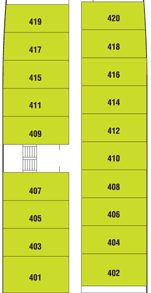
\includegraphics[angle=90]{images/rooms.png}
\caption{A small section of a ship deck}
\label{fig:rooms}
\end{figure}

\begin{figure} [h]
\centering
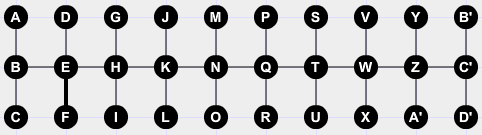
\includegraphics{images/simple.png}
\caption{The graph representing the ship deck}
\label{fig:simple}
\end{figure}

The ships are created from blueprints from ships currently in operation. They are modeled as graphs, nodes represents rooms and lines represents passages between rooms. Small rooms are represented by a single node as the layout of the room is fairly simplistic and the time it takes to move across the room is fairly predictable as long as the room is not crowded. Figure \ref{fig:rooms} shows a section of a ship deck with several rooms leading out into a hallway connected to a set of stairs. Figure \ref{fig:simple} shows a graph representing the same section. It is worth noting that while small rooms can be represented with a single node the hallway is represented by multiple nodes as a passenger exiting room 419 is far away from a passenger exiting room 401.

Complex or large rooms are represented by multiple interconnected nodes so each part of the room can be individually configured to better represent the room. Rooms like the dining room in the MS Reflection, as seen in figure \ref{fig:dining}, would need several nodes as the time it takes for the people close to the exit to evacuate are vastly different from the time it takes for the people sitting in the middle of the room to evacuate. Figure \ref{fig:complex} shows a representation of the dining room. 

\begin{figure} [h]
\centering
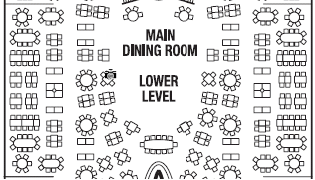
\includegraphics{images/Dining.png}
\caption{The dining room in the cruise ship MS Reflection}
\label{fig:dining}
\end{figure}

All rooms have a few characteristics associated with them. First is the room capacity, meaning the amount of people that can move across the room before they start to slow each other down. Second is the chance of death, this number will change over time as the fire spreads throughout the ship. Third is the type of room, for instance stairs, hallway, gift shop etc. Fourth is the size of the room, which in turn will determine the time it takes to traverse the room. Additionally there are a exit nodes where all passengers gather before lifeboat embarkation. These are the nodes the algorithms attempts to guide the passengers towards.

\begin{figure} [h]
\centering
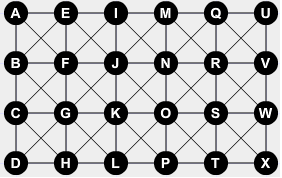
\includegraphics{images/complex.png}
\caption{A simple representation of the dining room of the MS Reflection}
\label{fig:complex}
\end{figure}

It became clear to us that using pathfinding algorithms to find the shortest route of small vessels were unnecessary as  there often would be only a single route to take and all passengers would be confined to one or two large areas where personnel easily could guide the passengers to safety. The algorithms are only helpful given multiple routes and rooms. 

\subsection{Human Behavior}

% Varying chance of panic

At the beginning of the simulation we assume that all passengers have access to a smart phone, which will show them the way out, and that they are following directions. Additionally, no passengers will start the simulation in a panicked state. However at certain time intervals a check is made to determine whether a passenger panics or not. Close proximity to fire, a high density of passengers or other panicked passengers increase the chance that they themselves will panic. When in a panicked state the passengers run out of the ship the same way they walked into it. Even if that path is significantly more dangerous.

Passengers with family members onboard the ship can enter a search state where they walk in a random pattern searching for family members until they find them, at which point they can resume following directions. The passengers can spot family members within their own node and any adjacent nodes. Family members that are not in a search state will also group up if they are within spotting range. In this case the family member that is further along the escape path will wait for the other family member to catch up.

Furthermore, family members will stick together and the algorithms will make no attempts to split up a family and send them in multiple directions. Thus whenever a passenger is moved the program checks if a family member is close-by, and if so they are moved in the same direction.

\subsection{Algorithms}
The simulation starts by igniting between one and three fires. There is a time delay between the time the fire starts and the time the passengers begins to move. This delay is meant to account for the time it takes to react to the alarm, retrieve the smart phone and understand the directions given. Fires spreads faster between floors than along them. The speed of the fire depends on the ship materials and access to oxygen, thus we run the simulations with varying speeds to observe how the algorithms perform. The larger the fire is, the faster it spreads to the neighboring nodes. Additionally deadly smoke will spread further and faster than the fires. 

When the fire starts either the fire system is able to track the position of the fire or the electric system have been compromised and the ship is in a dead ship condition where tracking the progress of the fire is impossible. If there are no information about the location of the fire then the safest possible route is likely the quickest one. Thus we decided upon 4 different possible configurations of the algorithms, to test if different configurations perform better in different scenarios. First they can prioritize distance and selecting the shortest path. Second they can prioritize safety and completely ignore the distance to the exit. Third it can combine the two variables, valuing them equally or differently. Fourth it can first sort the paths based on one variable and then only sort based on the other variable if there is a tie. For instance if there are two equally safe paths the shortest one is chosen.

The speed of the passengers is based on two factors, the type of room and the amount of people in the room. Passengers in a crowded flight of stairs will move significantly slower than a passenger in an empty corridor. These numbers are gathered from IMO's estimation on passenger speed during evacuations \cite{speed}. Given a node of 4 meter length and a passenger speed of 1 m/s the passenger will naturally have traversed the node after 4 seconds. It is worth mentioning that the passenger will not move within the node itself, up to 4 seconds into the simulation the passenger is located in the initial node and at 4 seconds the passenger is then moved to the next node.











    \chapter{Results}
\label{ch:testing}

\section{Simulation data}
In our testing we ran the simulation from 200 to over 1000 iterations, as there was no significant difference from 200 to 1000 iterations we did most of the simulations to 200 iterations.

The number of passengers was set to the ship maximum number of passengers stated on Cruisedeckplans LLC\cite{cruseships} website.

The hazards on-board the ship was set to increase at every second time step, both in number of nodes and how deadly it was in a particular node. In ACO, at each time step, the passengers was set to use 200 ants to find their way trough the ship, and each ant holding 200 pheromones to spread around. Also in each of these simulation, one fire was started, however some times it was randomly chosen one to three times.

In some of our simulation, it happens that a passenger would walk on board the ship for much longer then 300 time steps. However we have cut the graph at 300 time steps, as this would show more details in the graph about the algorithms and the average number of survives past 300 did not change.


\subsection{Celebrity Xpedition}

\begin{figure} [h]
\centering
\hspace*{-5.5in}
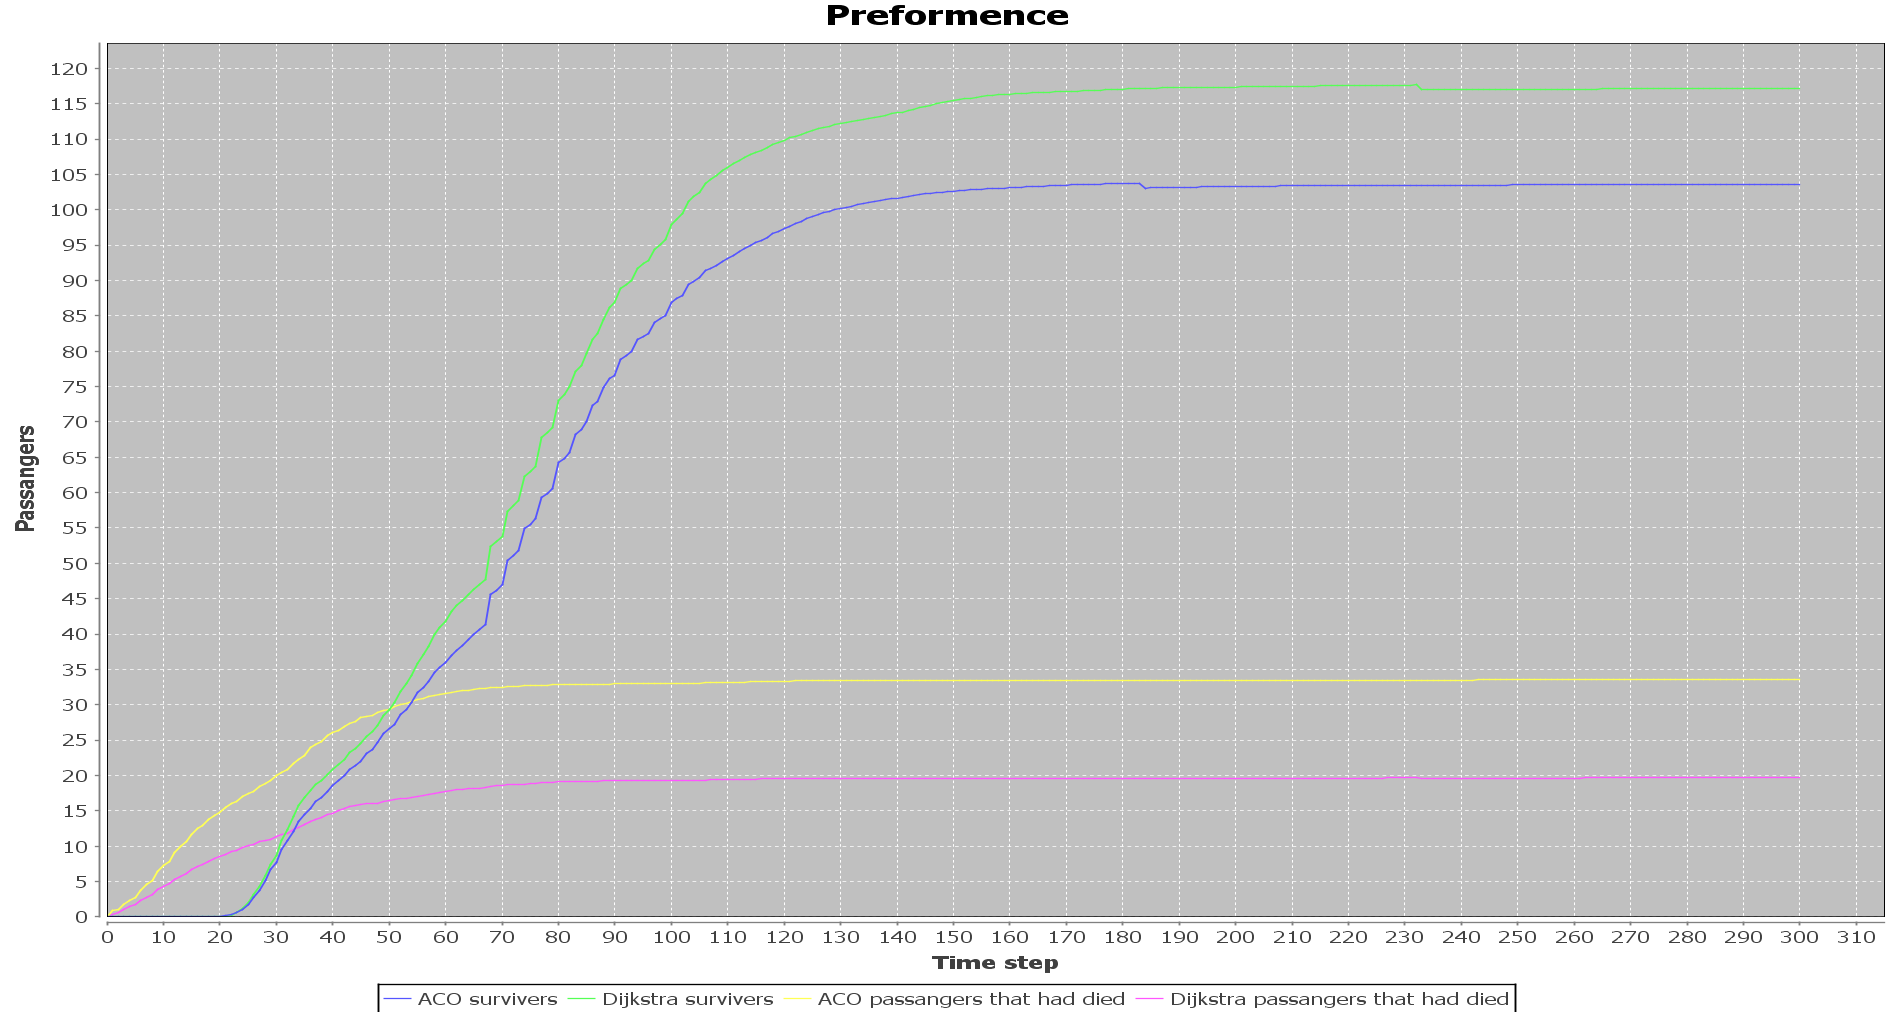
\includegraphics[scale=0.35]{images/Graph using 200 rounds 140 passangers and shortest first one hazzard.png}
\caption{The graph showing survives and deaths over a time table}
\label{fig:celebShortest}
\end{figure}

In \ref{fig:celebShortest} you can see how well the different algorithms did. In both cases we only used one hazard(Fire) that spread on board the ship. As shown in the graph, Dijkstra outperforms ACO in both early and late stages of this graph. In the beginning there are more passengers dying to ACO chosen path then there is in Dijkstras choesen path, a good sign that both are finding different paths. As shortest path is measured in shortest time needed rather then shortest way to exit, it may be that Dijkstra spread the passangers more out then ACO.

Even when more passengers are dying at the beginning of the simulations, they both have the same boost in saved passengers at each time step.

The biggest problem for ACO over Dikstra is avoiding the hazards. Shown in the graph you can see that the death toll for ACO increases faster then Dijkstras death toll.

\begin{figure} [h]
\centering
\hspace*{-5.5in}
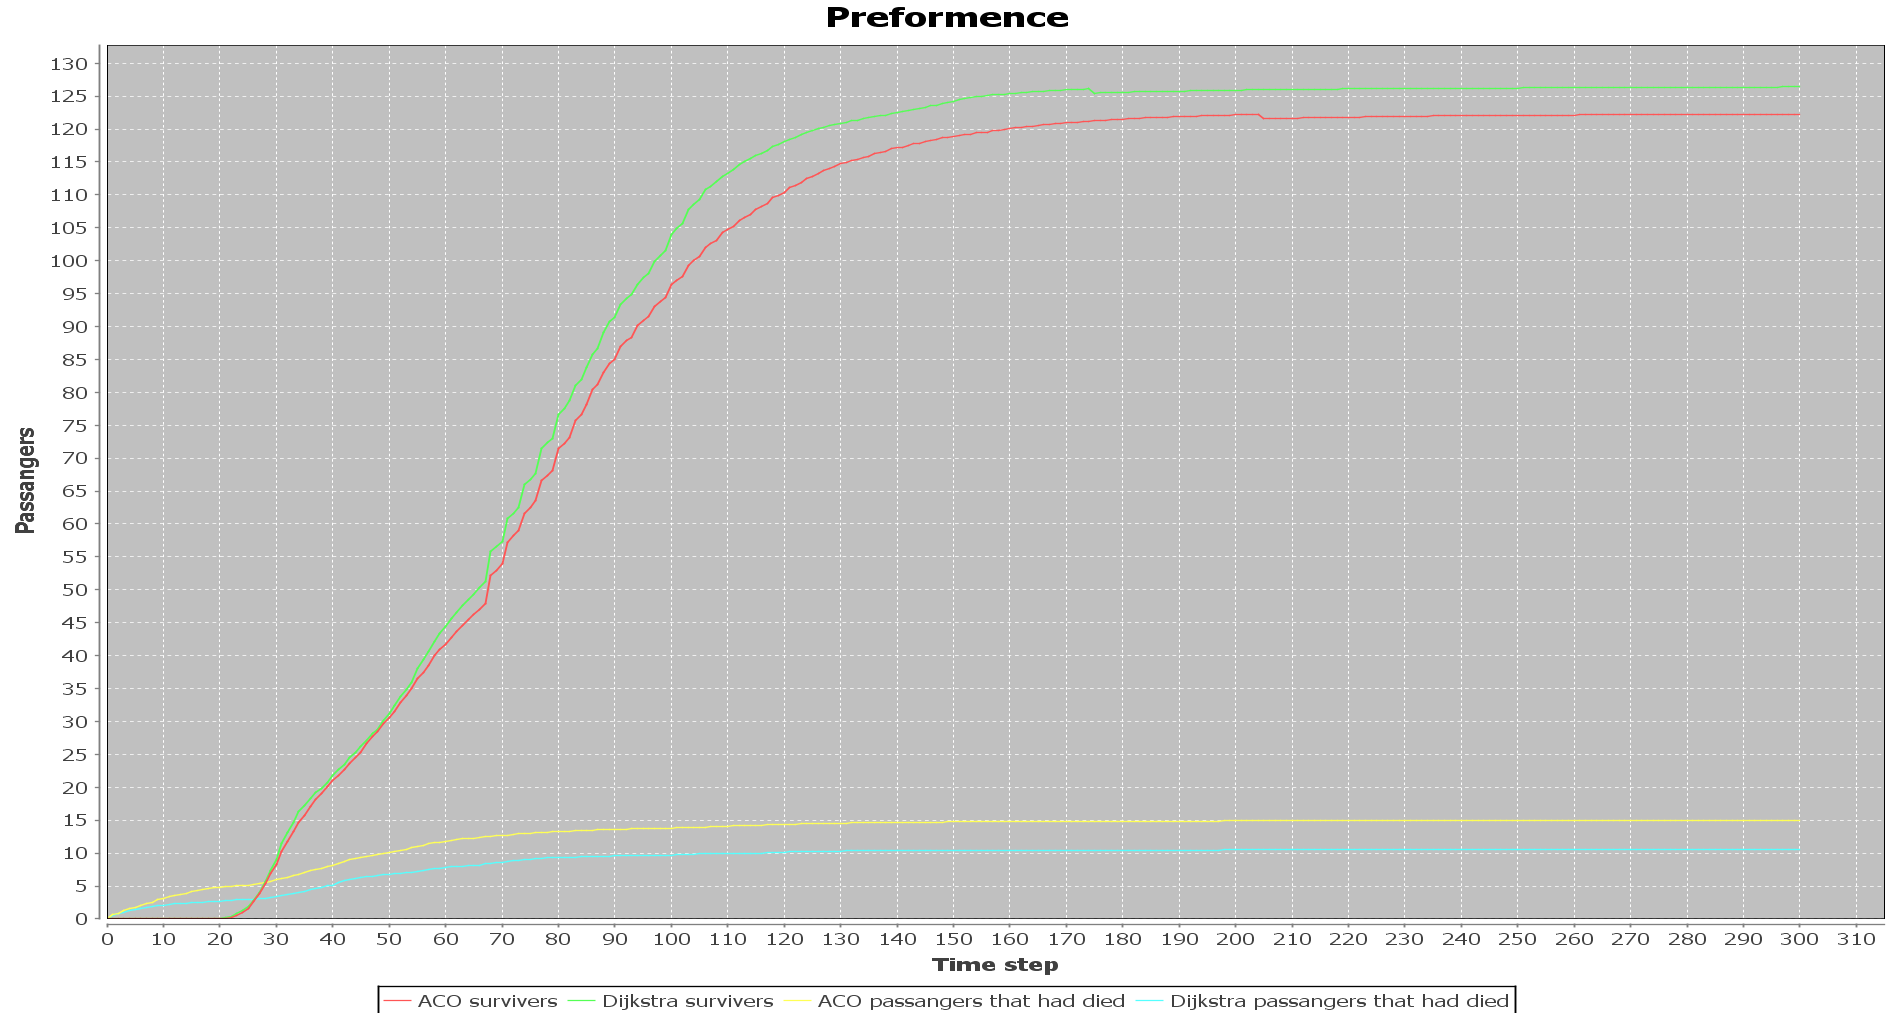
\includegraphics[scale=0.35]{images/Graph using 200 rounds 140 passangers and safest first one hazzard.png}
\caption{The graph showing survives and deaths over a time table}
\label{fig:celebSafty}
\end{figure}

In \ref{fig:celebSafty}, we are using the same parameters as the first one, only difference is that we are looking after the safest path rather then the shortest path for the passengers. It is clearly shown that the death toll on the passengers is far lower then the previous one.
However Dijkstra proves yet again to outperform ACO in this instance. After about 30 time steps Dijkstra starts to pull ahead of ACO in number of passengers it have guided to the lifeboats. Even in number of deaths it is shown that Dijkstra is better at avoiding them.

If you look at Dijkstra in both cases, the number of deaths when looking after the safest path is 50\% less when looking for the shortest path.

As mention earlier that the number of rounds above 200 did not matter may be shown in the two graphs below, both of them have the same set of parameters, only to have 1000 iteration instead of 200.

\begin{figure} [h]
\centering
\hspace*{-5.5in}
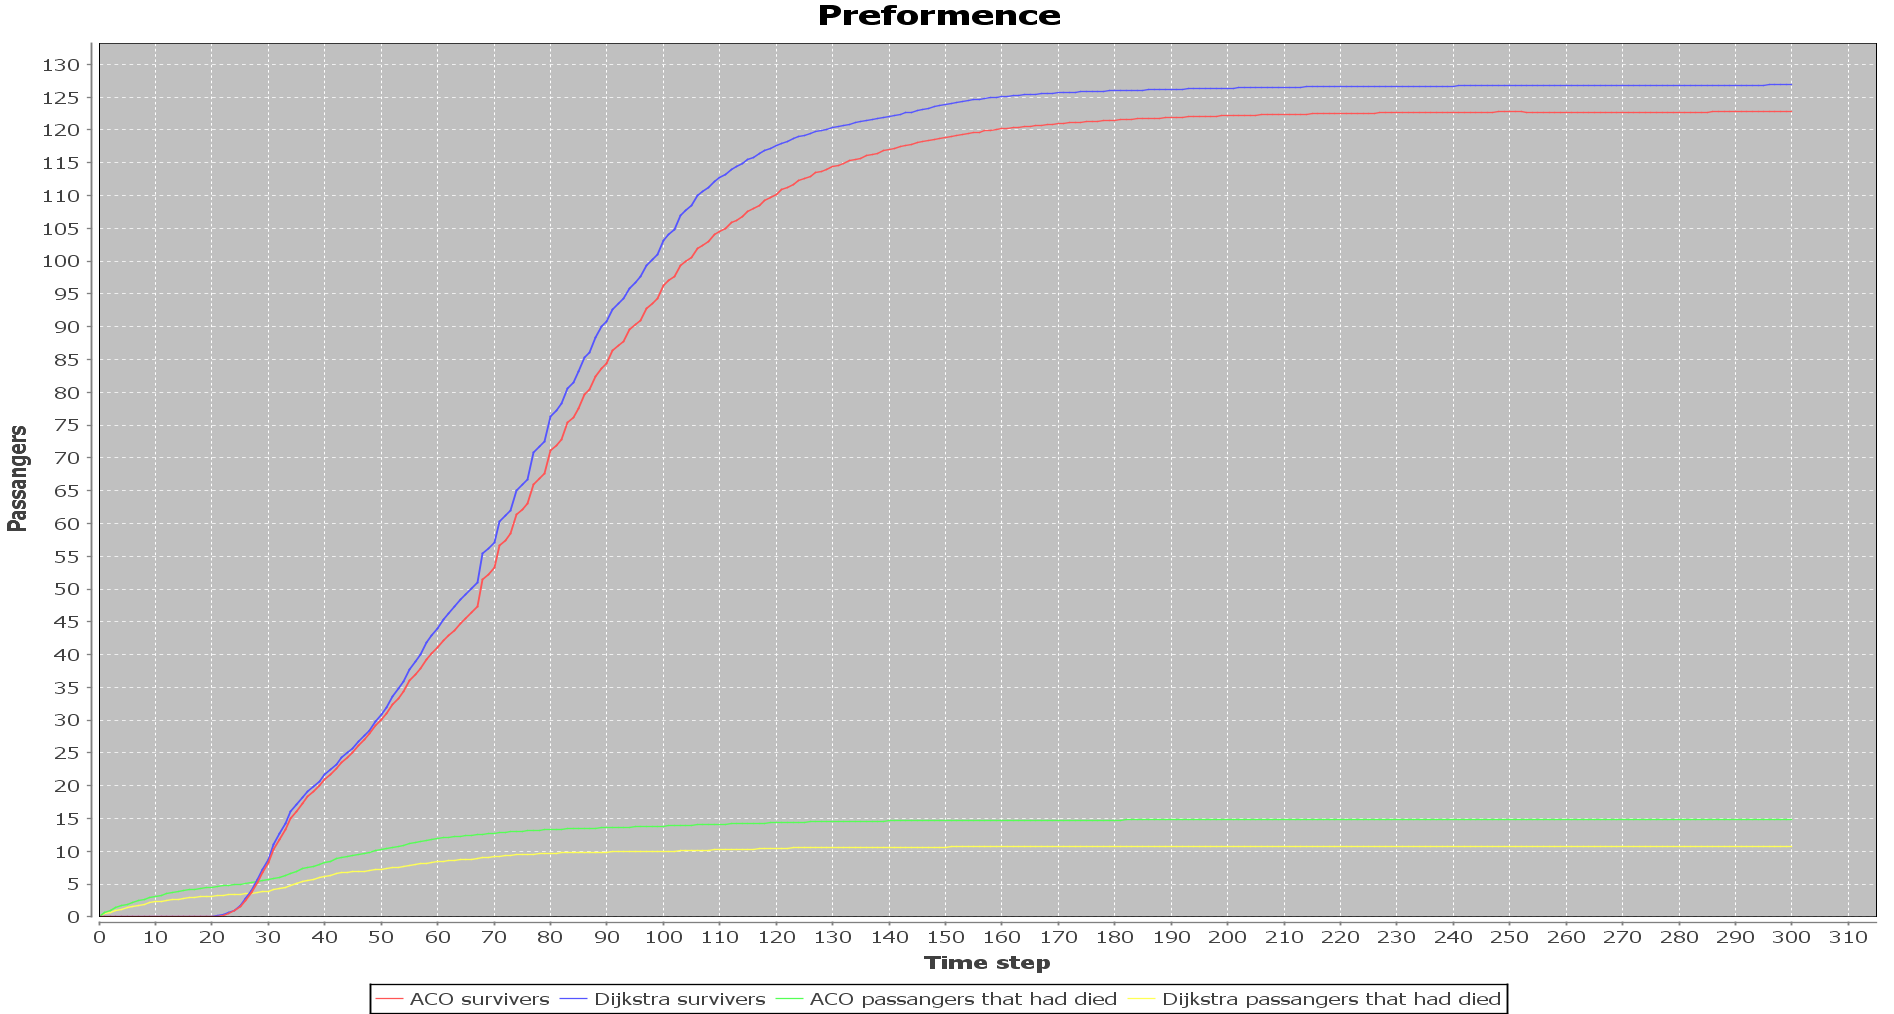
\includegraphics[scale=0.35]{images/Graph using 1000 rounds 140 passangers-safest path and one fire.png}
\caption{The graph showing survives and deaths over a time table}
\label{fig:celebSafty1000round}
\end{figure}

This graph is 1000 iterations of the simulation when looking for the safest way for each passengers. The next one shows the same thing, only looking for the shortest way to an exit.

\begin{figure} [h]
\centering
\hspace*{-5.5in}
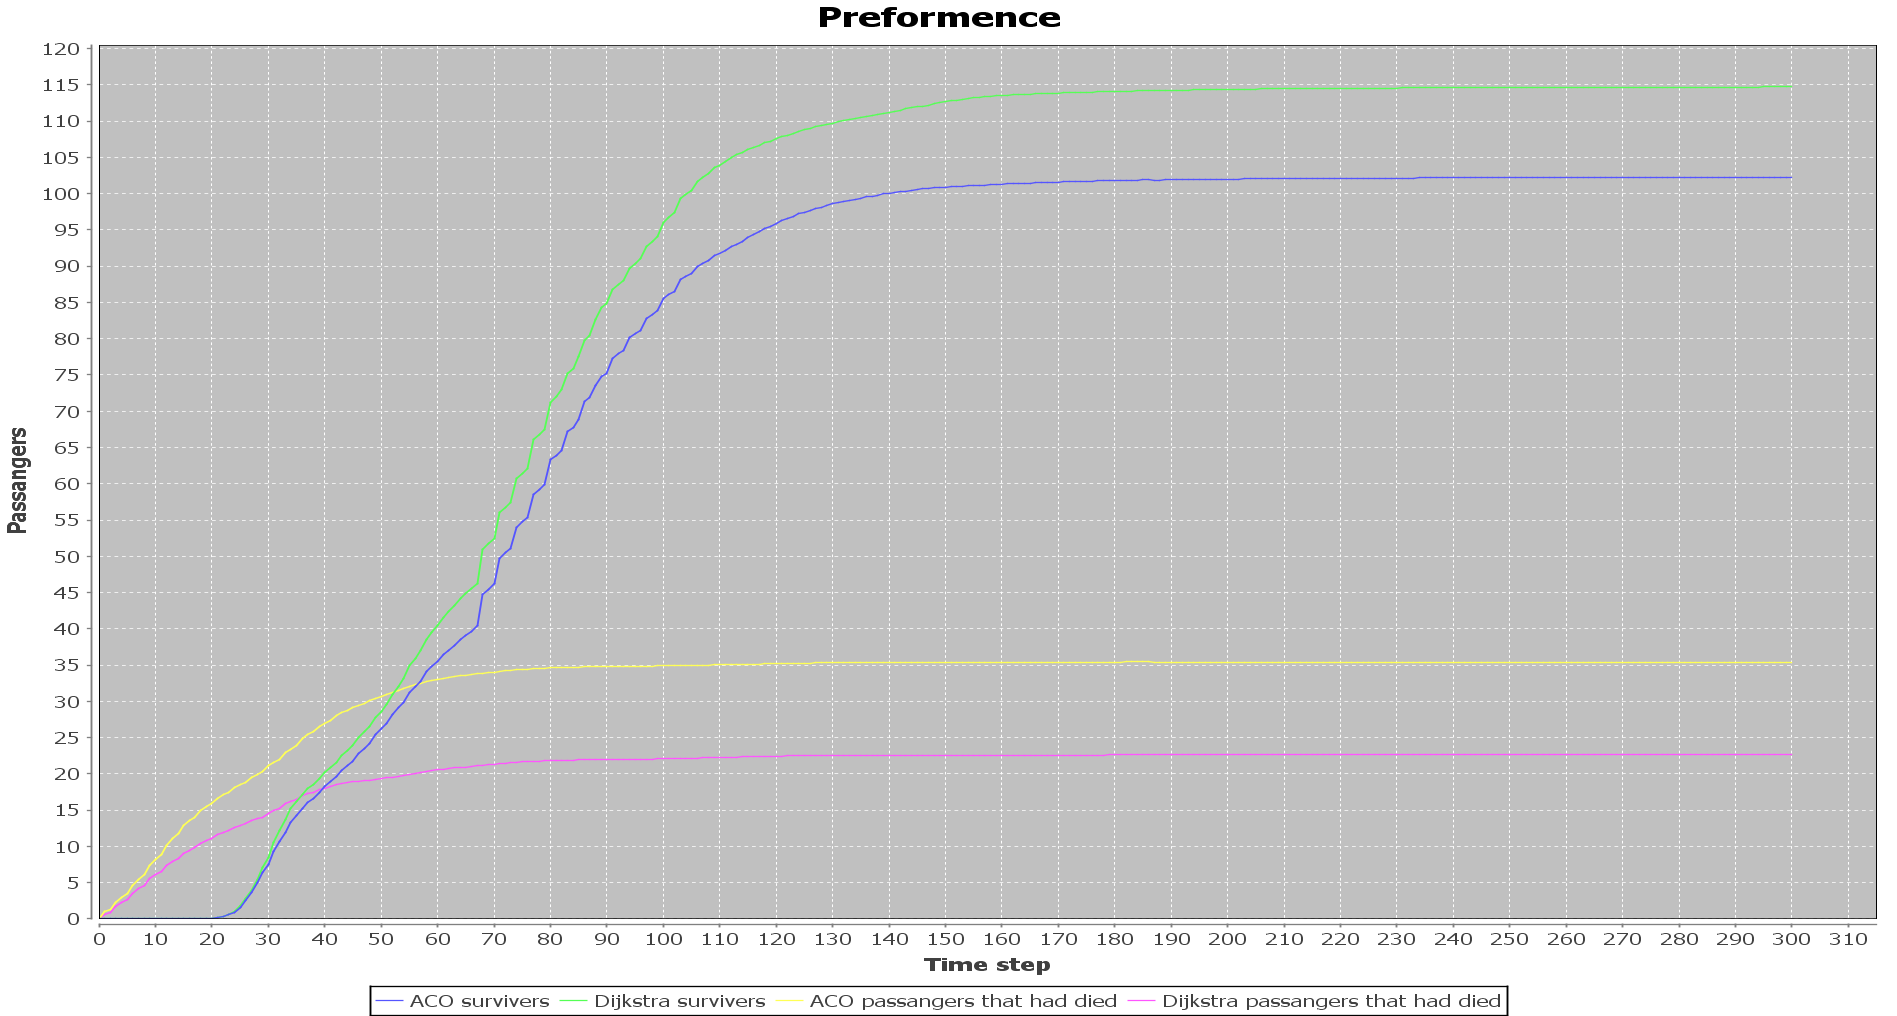
\includegraphics[scale=0.35]{images/Graph using 1000 rounds 140 passangers-shortest path and one fire.png}
\caption{The graph showing survives and deaths over a time table}
\label{fig:celebShort1000round}
\end{figure}


In \ref{fig:celebShortPherInEdges} and \ref{fig:celebSafePherInEdges} we tested what would the difference be if we used pheromones in edges rather then in the node themselves, this showed that the ACO preformed better then our other simulations. It was compared to Dijkstra to control that there was not something special happening. The main difference is when looking for the shortest path rather then the safest. When looking for the safest there are only some small difference in both simulations.

\begin{figure} [h]
\centering
\hspace*{-5.5in}
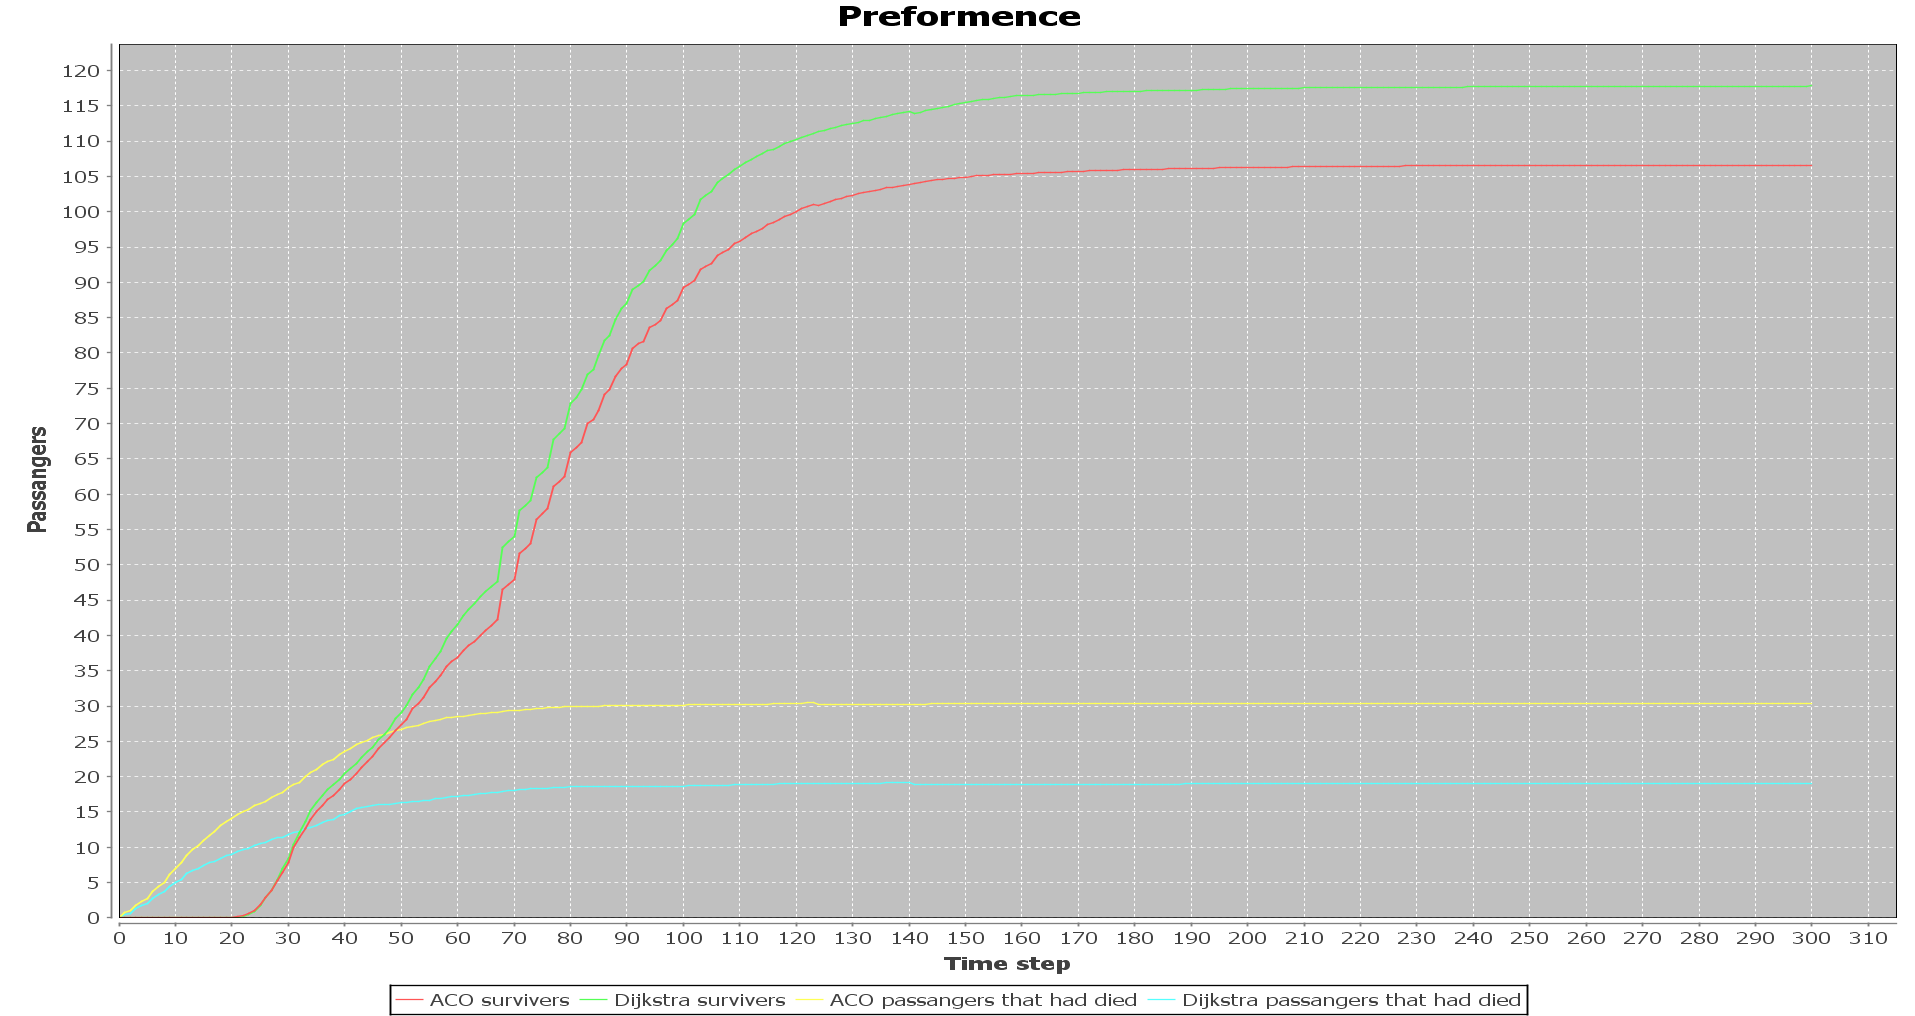
\includegraphics[scale=0.35]{images/Graph using 200 rounds 140 passangers and shortest first one hazzard and ACO having pheremons in edges.png}
\caption{The graph showing survives and deaths over a time table}
\label{fig:celebShortPherInEdges}
\end{figure}

\begin{figure} [h]
\centering
\hspace*{-5.5in}
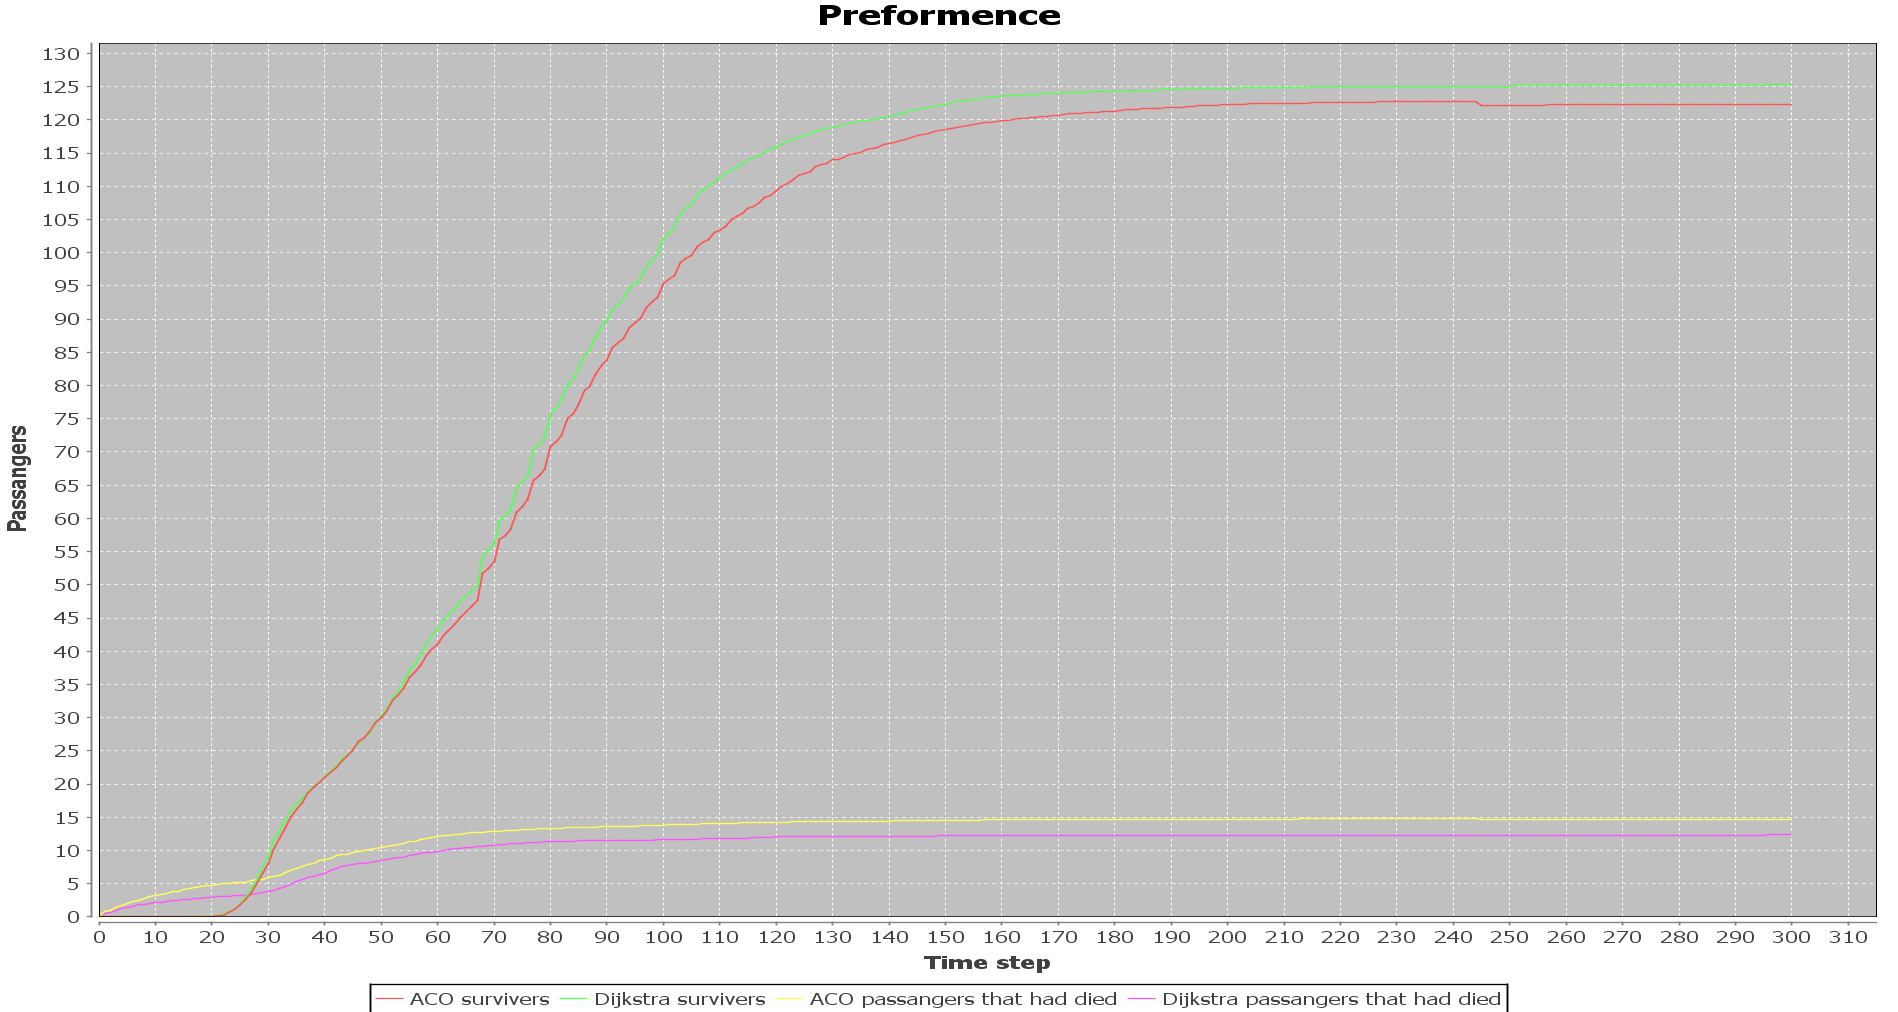
\includegraphics[scale=0.35]{images/Graph using 200 rounds 140 passangers and safest first one hazzard and ACO having pheremons in edges.png}
\caption{The graph showing survives and deaths over a time table}
\label{fig:celebSafePherInEdges}
\end{figure}
    \chapter{Conclusion and further work}
\label{ch:conclusion}

\section{Conclusion}

The goal of the project was to both simulate a crisis on board a ship and find safe passage of the ship for the passengers. Our focus was on an Ant Colony Optimization pathfinding algorithm which performance was measured against Dijkstra's pathfinding algorithm.  The algorithms were tested in a dynamic crisis environment where passengers could panic, fire could spread and high occupant density could hamper movements. We worked on a solution where the ships were modeled as graphs with nodes representing rooms and edges representing transitions between rooms. At the start of the simulation fire would break out and it would spread at an increased rate as time passed. Basic human behavior was implemented by giving each passenger an increased chance to panic when in close proximity to danger or other panicking passengers. Additionally family members would stick together and the system would make no attempts to send them in different directions. 

The simulations showed that in small graphs Dijkstra's algorithm would performed better. The time it takes for ACO to calculate a safe passage is tied to the amount of ants the algorithm runs, and a certain amount of ants is necessary to ensure a good result. Thus Dijkstra's algorithm is both faster and saves more lives in a simulation using a small graph. In larger graphs ACO performs faster than Dijkstra's algorithm as the increasing number of edges and nodes impacts Dijkstra's algorithm more than ACO.

As the project is over we can state that the it met the requirements. The algorithms were tested under the conditions that were planned and produced good results. The system is not ready for deployment but it does show that there are benefits to such a system if it were completed. ACO performed well under certain conditions and could be used as the pathfinding algorithm in a future system.

\section{Further Work}

As stated in the introduction, the goal of our work was not to create a fully functional system, one that could be deployed in a real crisis. To do so one would need to expand upon our solution. First the system would need to be able to identify all phones in the crisis area. This is necessary to both be able to identify which phone to send directions to and to track the movements of all passengers. The movements of the passengers would be tracked using the GPS in the phone. Second the system needs to be able to send directions to the phones. One can not expect every passenger to install an app, thus the system would need a way to take over the phone and show the image of the escape route. 

Third the system would need a way to alert all passengers that evacuation routes will be sent to their phones. For instance by displaying messages on TV screens and announcing it over the ships audio systems. In case of electric failure the TV screens and audio system would need to have backup batteries.  Fourth, not all passengers carry smart phones thus the system should send the directions to one phone and have the owner guide the surrounding passengers. In the case where there are passengers that are not carrying a smart phone the system would need an alternate way of tracking passengers, possibly by using on board cameras.

Fifth the system needs would need a database of all ship models. This could be done by creating a parser that transforms ship blueprints into graphs. Any company that wished to have this evacuation system installed would have to submit blueprints of their ships. Sixth the system would need to calculate the routes as fast as possible and as safe as possible. This could be solved by a combination of using massive computer power, optimizing the algorithm and spending a finite amount of time calculating each route.


    \chapter*{Acknowledgements}%
\addcontentsline{toc}{chapter}{Acknowledgements}%

We would like to thank our supervisors Morten Goodwin and Ole-Christoffer Granmo. They have provided us with motivation, smart suggestions and constructive feedback whenever we have needed it. Without them this project would not have been completed. 

    \begin{singlespace}
        \bibliographystyle{IEEEtranS}
        %\bibliographystyle{plain}
				%\bibliographystyle{apalike}
        \bibliography{bib/web}
    \end{singlespace}

    \printglossary   

\end{document}

